\section{Redox-Reaktionen}

\subsection{Grundlagen}
    \begin{minipage}{0.5\linewidth}
        Reduktionsmittel (RM) = $e^{-}$-Spender

        Oxid\tikz[baseline=(text.base)]\node[fill=orange, fill opacity=0.3, text opacity=1, rounded corners, inner sep=2pt, minimum height=5pt] (text) {a};tion = $e^{-}$-Abg\tikz[baseline=(text.base)]\node[fill=orange, fill opacity=0.3, text opacity=1, rounded corners, inner sep=2pt, minimum height=5pt] (text) {a};be

        = Erhöhung der OZ
    \end{minipage}
    \hfill
    \begin{minipage}{0.5\linewidth}
        Oxidationsmittel (OM) = $e^{-}$-Akzeptor

        Red\tikz[baseline=(text.base)]\node[fill=green, fill opacity=0.3, text opacity=1, rounded corners, inner sep=2pt, minimum height=5pt] (text) {u};ktion = $e^{-}$-A\tikz[baseline=(text.base)]\node[fill=green, fill opacity=0.3, text opacity=1, rounded corners, inner sep=2pt, minimum height=5pt] (text) {u};fnahme

        = Erniedrigung der OZ
    \end{minipage}

    % Eine Reaktion ist eine Redox-Reaktion, wenn die Oxidationszahlen der Atome der Edukte nicht die selben sind wie die Oxidationszahlen der Atome der Produkte.
    
    \begin{minipage}{0.5\linewidth}
        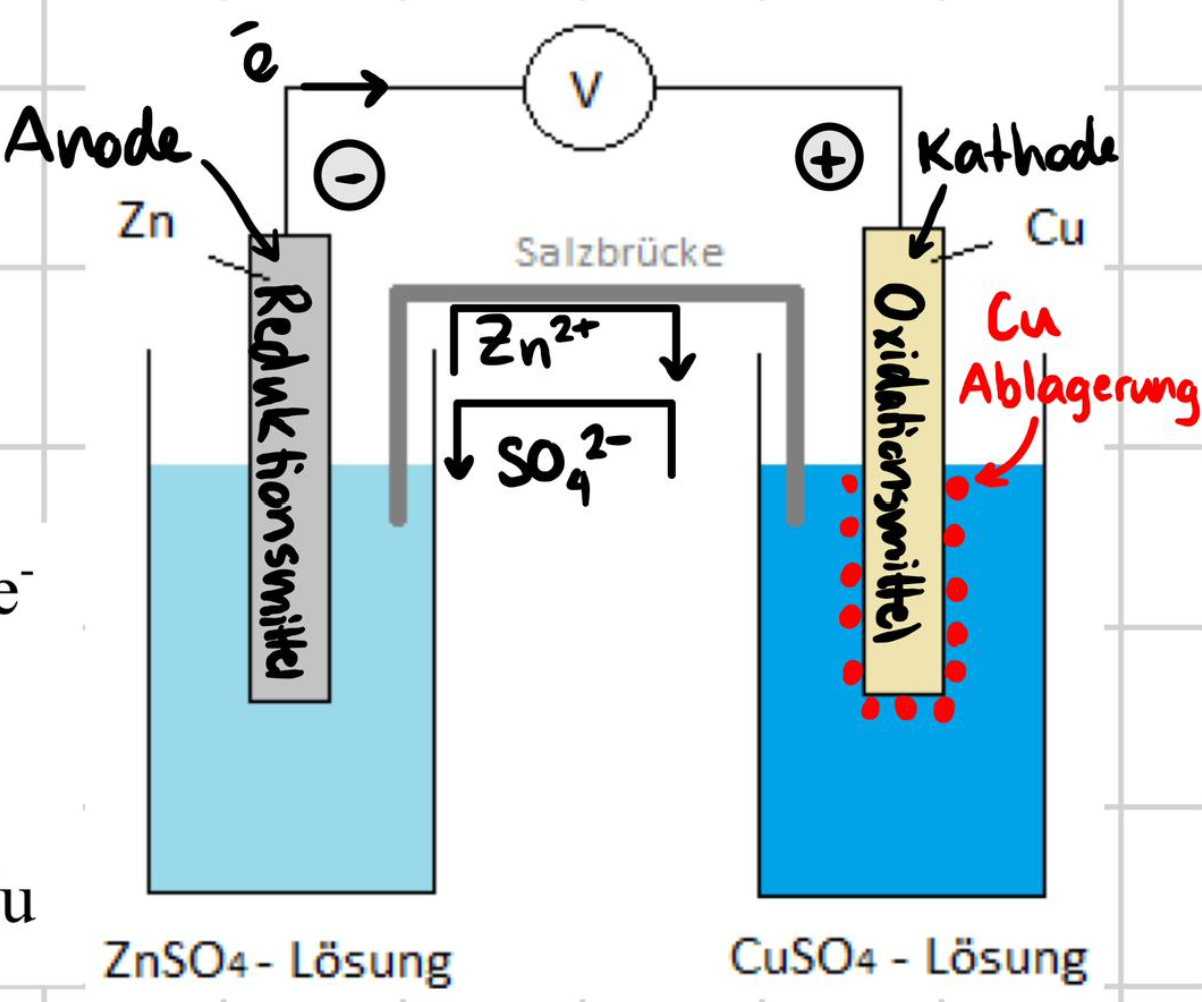
\includegraphics[height=4cm]{pictures/Galv.png}
    \end{minipage}
    \hfill
    \begin{minipage}{0.5\linewidth}
        Oxidationszahlen:
        \begin{itemize}
            \item[\textbf{R1}] OZ elementarer Stoffe ist Null
            \item[]            \ce{O_2^0, Cl_2^0}
            \item[\textbf{R2}] OZ einatomiger Ionen = Ionenladung
            \item[]            \ce{Na^+} : +I, \ce{Fe^{2+}} : +II
            \item[\textbf{R3}] Bei Molekülen;
            \item[]            Bindungselektr. beim neg. Atom
            \item[\textbf{R4}] Summe aller OZ = Ladung des Teilchens
        \end{itemize}
    \end{minipage}
    % Aufgrund der \textbf{Standartpotenziale} der Metalle Zn und Cu herrscht eine ``Spannun'', welche die Reaktion ermöglicht. 
    % Das \textbf{\ce{Zn^0}} wird an der Anode zu \textbf{\ce{Zn^2+}} oxidiert (\ce{e^-}-Abgabe), \textbf{\ce{Zn^0}} dient somit als Reduktionsmittel. 
    % Die Elektronen werden an die Kathode abgegeben, wo \textbf{\ce{Cu^2+}} aus der Lösung zu \textbf{\ce{Cu^0}} reduziert (\ce{e^-}-Aufnahme) wird. 
    % \textbf{\ce{Cu^2+}} dient somit als Oxidationsmittel. Damit die Lösungen jeweils ungeladen bleiben, wandern über die Salzbrücke 
    % \textbf{\ce{Zn^2+}-Ionen} und \textbf{\ce{SO4^2-}-Ionen}.
\subsection{Redoxpotential}
    Redoxpotential $\to$ auslesen aus Redoxreihe ganz rechts 
    
    Gemessen gegenüber Wasserstoff-Elektrode

    Abhängig von: pH, Druck, Ionenkonzentration, Temperatur $\to$ \textbf{Nernst-Gleichung:}

    % Das Redoxpotential einer Halbzelle kann aus der Redox-Reihe ausgelesen werden (ganz rechts). Dieses Potenzial wurde jeweils 
    % gegenüber einer Standart-Wasserstoff-Elektrode gemessen.
    
    % Das Redoxpotential ist jedoch von pH, Druck, Ionenkonz und Temperatur abhängig. Potenziale bei Nicht-Standardbedingungen können 
    % mit folgender GLeichung berechnet werden.


    \begin{minipage}{0.4\linewidth}
        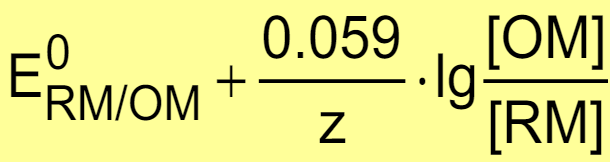
\includegraphics[width=\linewidth]{pictures/Nernst.png}
    \end{minipage}
    \hfill
    \begin{minipage}{0.55\linewidth}
        \begin{itemize}
            \item z = Anz. \ce{e^-} die pro Atom übergeben werden
            \item \ce{[OM]} = konz. OM in mol/L
            \item \ce{[RM]} = konz. RM in mol/L, bei Metallen 1
        \end{itemize}
    \end{minipage}


     \begin{minipage}{0.65\linewidth}
        Inkl. pH-Wert:

        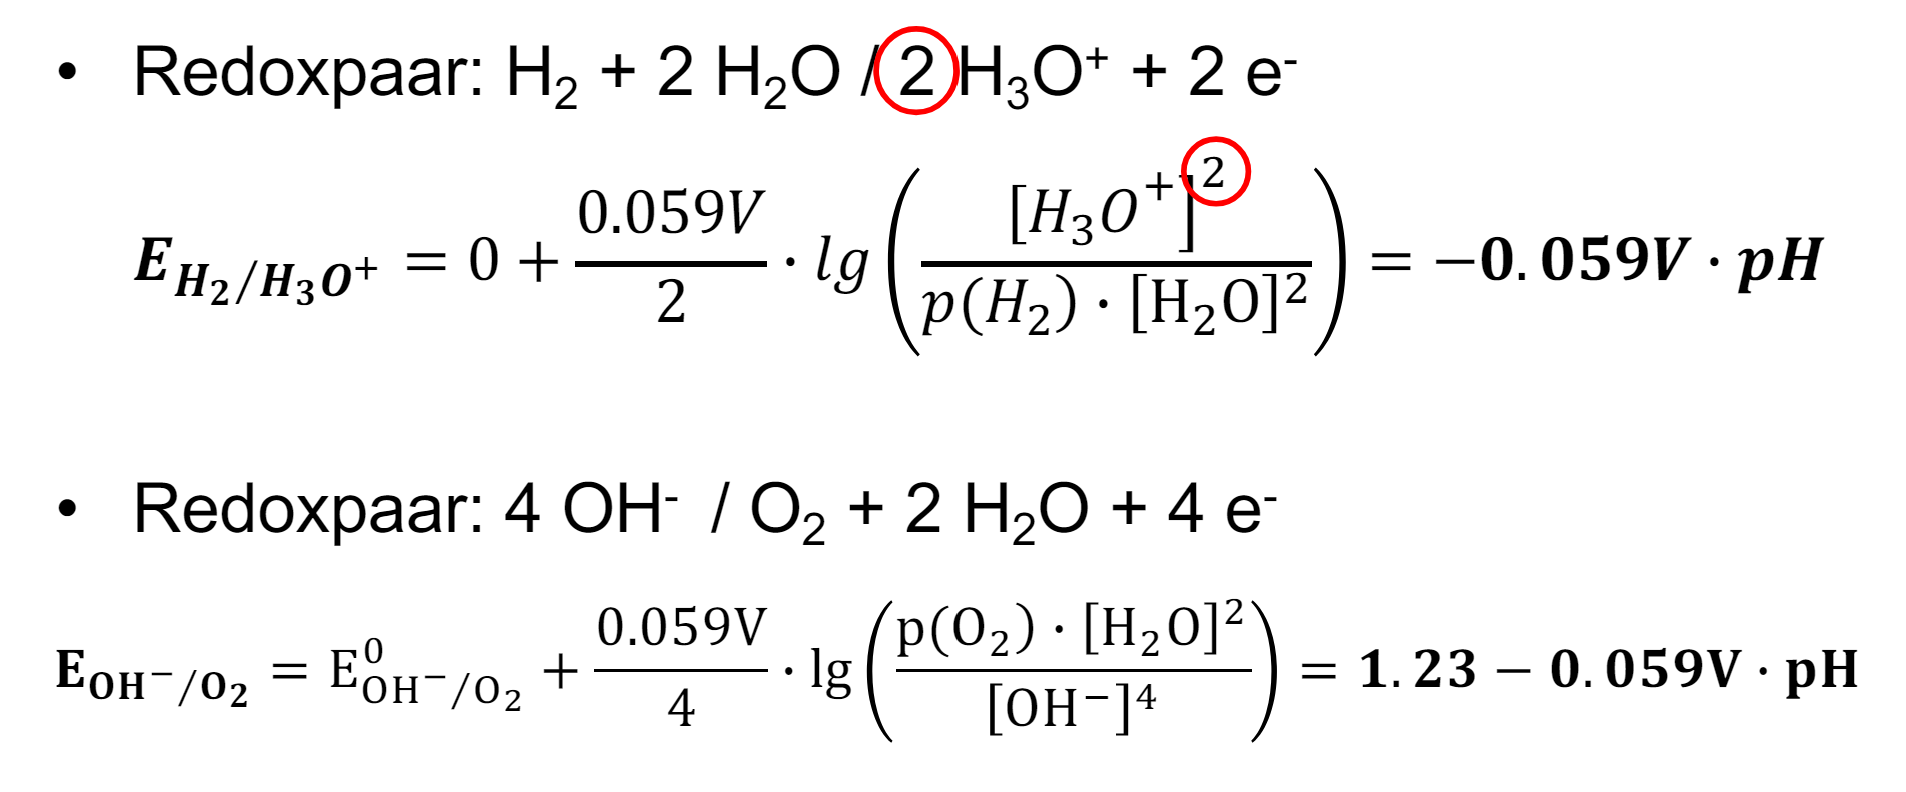
\includegraphics[height=2.8cm]{pictures/Nernstph.png}
    \end{minipage}
    \hfill
    \begin{minipage}{0.3\linewidth}
        Edle Metalle E > 0V
        \begin{itemize}
            \item Gold, Silber
            \item Platin, Palladium
        \end{itemize}
        Unedle Metalle E < 0V
        \begin{itemize}
            \item Natrium, Lithium
            \item Eisen, Zink
        \end{itemize}
    \end{minipage}